\documentclass[a4paper,11pt]{report}

\usepackage{atbegshi}% http://ctan.org/pkg/atbegshi
\AtBeginDocument{\AtBeginShipoutNext{\AtBeginShipoutDiscard}}
%\newcommand{\makecell}[2][@{}c@{}]{\begin{tabular}{#1}#2\end{tabular}}
\usepackage[italian]{babel}
\usepackage{here}
\usepackage[T1]{fontenc}
\usepackage[utf8]{inputenc}
\usepackage{lmodern} 
\usepackage{textcomp} 
\usepackage{graphicx} 
\usepackage{amsmath}
\usepackage{amsthm}
\usepackage{amsfonts}
\usepackage{gensymb}
\usepackage{listings}
\usepackage{tabularx}
\usepackage{longtable}
\usepackage{float}
\usepackage{subfigure}
\usepackage{rotating}
\usepackage{cleveref}
%\usepackage[]{mcode}
%\usepackage{cancel}


\usepackage{listings}
\usepackage{color} %red, green, blue, yellow, cyan, magenta, black, white
\definecolor{mygreen}{RGB}{28,172,0} % color values Red, Green, Blue
\definecolor{mylilas}{RGB}{170,55,241}


\lstset{language=Matlab,%
    %basicstyle=\color{red},
    breaklines=true,%
    morekeywords={matlab2tikz},
    keywordstyle=\color{blue},%
    morekeywords=[2]{1}, keywordstyle=[2]{\color{black}},
    identifierstyle=\color{black},%
    stringstyle=\color{mylilas},
    commentstyle=\color{mygreen},%
    showstringspaces=false,%without this there will be a symbol in the places where there is a space
    numbers=left,%
    numberstyle={\tiny \color{black}},% size of the numbers
    numbersep=9pt, % this defines how far the numbers are from the text
    emph=[1]{for,end,break},emphstyle=[1]\color{red}, %some words to emphasise
    %emph=[2]{word1,word2}, emphstyle=[2]{style},    
}




\usepackage{mathrsfs}
\usepackage{color}
\usepackage[top=1.0in, bottom=1.5in, left=0.5in, right=0.5in]{geometry}
\usepackage{wrapfig}
\usepackage[normalem]{ulem}
\usepackage[toc, page]{appendix}
\usepackage{hyperref}
\graphicspath{ {Figure/} }
\makeatletter
\DeclareRobustCommand*\textsubscript[1]{%
  \@textsubscript{\selectfont#1}}
\def\@textsubscript#1{%
  {\m@th\ensuremath{_{\mbox{\fontsize\sf@size\z@#1}}}}}
\makeatother
%per togliere la parola capitolo dall'intestazione
\makeatletter
%\renewcommand\@chapapp{}
\makeatother

\title{\medskip
\begin{Huge}
\textbf{Politecnico di Milano}
\end{Huge}
\linebreak
\begin{figure}[ht]
\centering

\includegraphics[scale=1]{poli.jpg}
\end{figure}
\linebreak\linebreak
\begin{huge}
Visualizzazioni a fili di fumo 
\end{huge} 
\linebreak\linebreak  
\begin{LARGE}
Fluidodinamica Sperimentale 2016/17
\end{LARGE}
\linebreak\linebreak\linebreak\linebreak\linebreak}
\author{\begin{tabular}{l l}
Tommaso Ghidoni & 841839\\
\\\\\\
\end{tabular}}


\begin{document}
\pagenumbering{roman}
\pagestyle{empty}
\maketitle
\pagebreak
\tableofcontents
\listoffigures
\listoftables
\cleardoublepage
\pagenumbering{arabic}
\pagestyle{plain}
\pagebreak
\include{intro}
\chapter{Prova sperimentale}
\section{Galleria}
La prova è stata svolta nella galleria del vento adibita alle visualizzazioni del Politecnico di Milano. Questo modello viene usato per indagare correnti bidimensionali ed ha una camera di prova di dimensione \textasciitilde $550x300x40 mm$.
La generazione e immissione dei fili di fumo è svolta da un sistema integrato nella galleria: il generatore di fumi consiste in una resistenza che fa evaporare olio di parafina, mentre l'immissione è affidata ad un rastrello di cannule posto a circa 150 mm dall'asse di rotazione del profilo. La galleria è illuminata da lampade a fluorescenza poste nella parete superiore,mentre la parete rivolta verso l'osservatore è trasparente. \\
Il profilo in esame è un NACA0013 di corda $c = 150 mm$, la sua rotazione è comandata a mano tramite un sistema a pulegge. \\
La corrente ha una velocità asintotica stimata $U_{\infty} = 1.5 m/s$; considerando la viscosità cinematica pari  $\nu = 1.5*10^-5 m^2/s$ è possibile calcolare il numero di Reynolds della prova:

\begin{center}
\begin{equation}
Re = \frac{U_{\infty} * c}{\nu} = 15000
\end{equation}
\end{center} 

\section{Strumentazione}
I filmati sono stati acquisiti con una fotocamera \emph{Canon EOS600D} attraverso un obiettivo grandangolare EF18-55mm f/3.5-5.6; la camera ha un sensore \emph{CMOS} da 18 Mpixel in modalità foto e permette riprese fino a 50 \emph{fps}. La macchina è stata posizionata su un cavalletto in modo da eseguire riprese stabili e mantenere un allineamento costante.

\section{Acquisizioni}
Data la necessità di indagare diverse grandezze sono state eseguite cinque acquisizioni. La frequenza di shedding attesa è molto minore di 10 Hz; ciò ha permesso di acquisire il filmato anche con un framerate ridotto a 24 fps soddisfando comunque il teorema di Nyquist. 

\begin{table}[h]
\centering
\begin{tabular}{|c|c|c|c|c|}
\hline
Nome & FPS & Esposizione frame [s] & ISO  & Descrizione \\
\hline
9900 & 24  & 1/40            & 1600 & Incidenza nulla\\
\hline
9904 & 24  & 1/30            & 3200 & Avvio e Vortex shedding \\
\hline
9906 & 24  & 1/30            & 1600 & Vortex shedding \\
\hline
9911 & 50  & 1/60            & 3200 & Vortex shedding \\
\hline
\end{tabular}
\caption{Descrizione acquisizioni}
\label{tab: Acquisizioni}
\end{table}



\include{analisi_immagine}
\chapter{Confronto dati}
\section{Angolo di stallo}
Il numero di Reynolds della prova è particolarmente basso, per questo motivo polari sperimentali affidabili non sono presenti in letteratura. Per ovviare a ciò è stata calcolata numericamente la porzione del grafico $Cl-\alpha$ per angoli compresi tra 8° e 12° (con passo 1°), il calcolo è stato effettuato con \emph{Ansys Fluent} utilizzando $k-\omega SST$ come modello di turbolenza. Il massimo $C_p$ è stato ottenuto ad 11°, l'angolo di stallo numerico sarà quindi compreso tra i 10° e i 12°, il risultato è concorde con quanto osservato nella visualizzazione [fig: \ref{erostall} ].
\section{Numero di Strouhal}
Non sono state reperite prove sperimentali comparabili all'esperimento qui considerato, ma la condizione fortemente stallata esibita durante le acquisizione consente di paragonare il profilo ad un corpo tozzo. \\
A riguardo la letteratura è ricca di prove sperimentali eseguite sul corpo tozzo per eccellenza: il cilindro. \\

\begin{figure}[h]
\centering
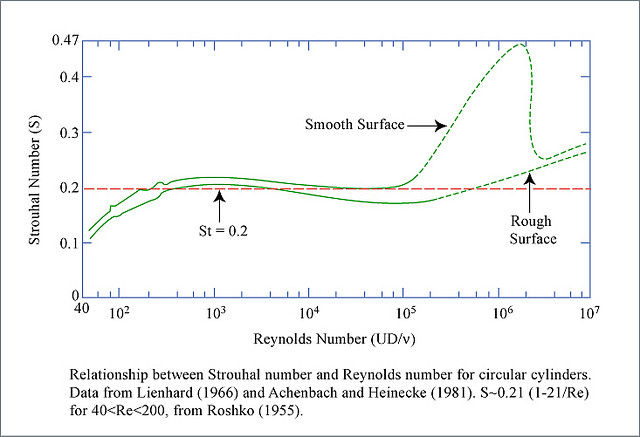
\includegraphics[scale=0.35]{Figure/str.jpg}
\caption{Numero di Strouhal nel cilindro}
\label{fig: Numero di Strouhal nel cilindro}
\end{figure}
Si può quindi assumere un numero di Strouhal pari a 0.2 [fig: \ref{fig: Numero di Strouhal nel cilindro}].

\begin{table}[h]
\centering
\begin{tabular}{|c|c|c|c|}
\hline
Strouhal teorico & Acquisizione 1 & Acquisizione 2 & Acquisizione 3\\
\hline
%$0.2$  & $0.222 \pm 0.004$   & $0.205 \pm 0.011$ & $0.194 \pm 0.011$\\
$0.2$  & $0.222$   & $0.205 $ & $0.194 $\\
\hline
\end{tabular}
\caption{Confronto numero Strouhal}
\label{tab: Confronto numero Strouhal}
\end{table}

Si nota come la seconda e la terza acquisizione [tab: \ref{tab: Confronto numero Strouhal} ] diano riscontro con il valore atteso; la prima,probabilmente a casua dell'incidenza minore, sovrastima il numero di Strouhal di oltre il dieci percento.

\section{Campo di moto e spessore scia}
E' stata eseguita una simulazione numerica nelle condizioni della prova [fig: \ref{fig: Campo di moto Fluent} ]. Il sotware utilizzato è \emph{Ansys Fluent},la mesh è dimensionata per riprodurre le dimensioni della camera di prova e, visto l'angolo di incidenza ridotta, è stato usato il modello di turbolenza ad 1 equazione di \emph{Spalart-Allmaras}. 

\begin{figure}[H]
\centering
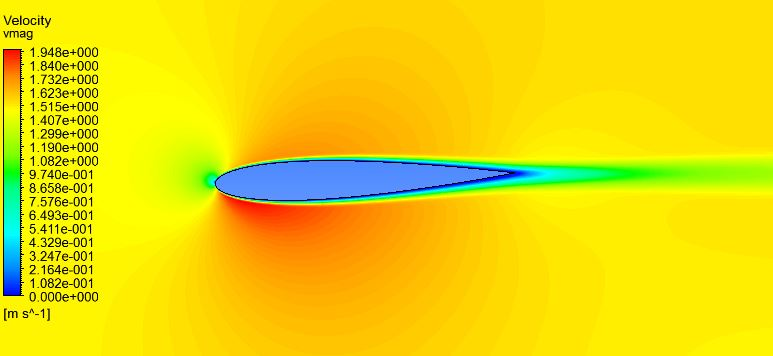
\includegraphics[scale=0.7]{Figure/CFD_wake.JPG}
\caption{Campo di moto calcolato con Fluent}
\label{fig: Campo di moto Fluent}
%\end{figure}

%\begin{figure}[h!]
\centering
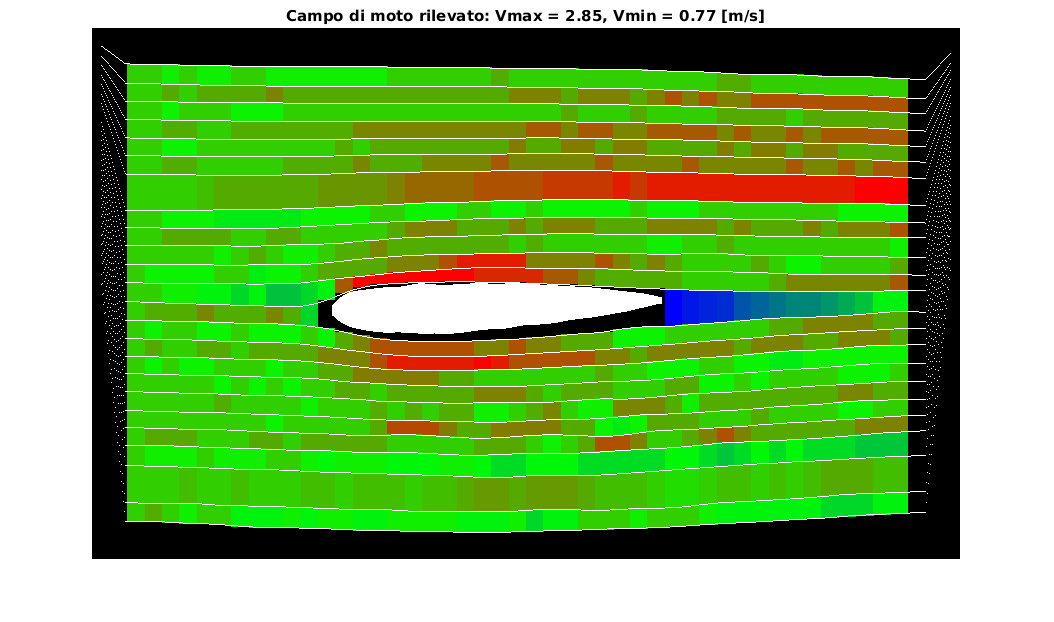
\includegraphics[scale=0.6]{Figure/v_field.png}
\caption{Campo di velocità calcolato da acquisizioni}
\label{fig: Campo di velocità calcolato}
\end{figure}

Il campo di moto simulato è stato campionato nelle coordinate ottenute dalla visualizzazione [fig \ref{fig: Campo di velocità calcolato} ], l'errore medio rilevato è 0.3 \emph{m/s}, con picchi di oltre $ 1 \emph{m/s}$. Da un confronto delle linee di corrente si nota che l'immagine elaborata è ancora distorta e,probabilmente, con un allineamento non perfetto nella fotocamera [fig: \ref{fig: Confronto linee di corrente}]. La distorsione è maggiore nella parte destra dell'immagine dove infatti si calcolano velocità non coerenti con il campo di moto: in particolare l'estremo destro del settimo tubo di flusso fa registrare una delle velocità più elevate dell'intero campo calcolato. 


\begin{figure}[H]
\centering
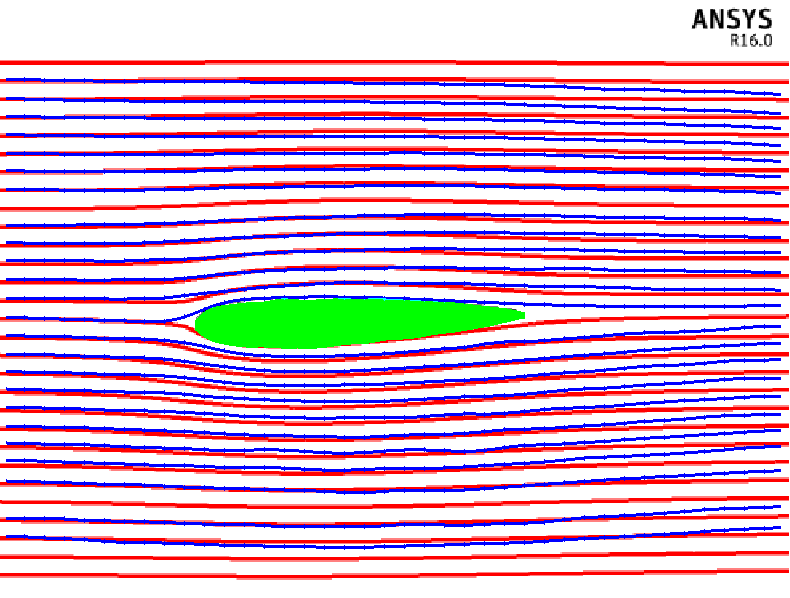
\includegraphics[scale=0.73]{Figure/Confronto.png}
\caption{Confronto linee di corrente Fluent (rosso) e linee di corrente acquisite (blu)}
\label{fig: Confronto linee di corrente}
\end{figure}


\begin{figure}[H]
\centering
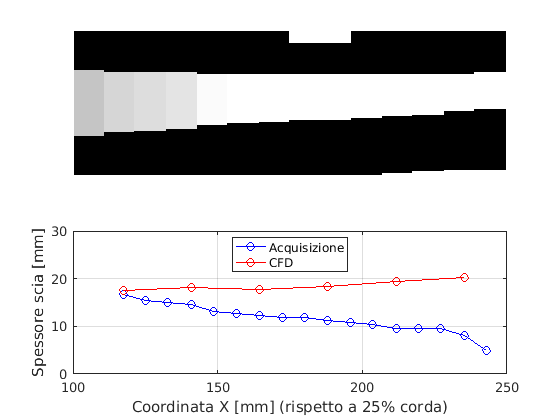
\includegraphics[scale=0.9]{Figure/scia_sper.png}
%\caption{Post interpolazione e filtraggio}
\caption{Scia visualizzata e andamento lungo coordinata X }
\label{fig: Scia rilevata}
\end{figure}

Stesso procedimento è stato effettuato per la scia, si nota che lo spessore oltre avere media quasi doppia ha anche un andamento opposto [fig: \ref{fig: Scia rilevata} ].\\

%t_{wake,video} = 11.61 \pm 3.9 [mm]
\begin{center}
$$ < t_{wake,video}(x) > = 11  [mm] $$
$$ < t_{wake,CFD}(x) >   = 18  [mm] $$
\end{center}


\chapter{Conclusioni}
Le misure qualitative dell'incidenza allo stallo e del numero di Strouhal sono soddisfacenti. \
Il campo di moto stimato presenta un errore medio elevato con valori massimi inacettabili anche solo per una stima qualitativa. La causa principale è da attribuirsi alla distorsione dell'immagine ed a un non perfetto allineamento della fotocamera [vedi fig \ref{fig: Confronto linee di corrente}].
Altri aspetti della prova sono migliorabili:
\begin{itemize}
\item l'esperienza acquisita durante l'elaborazione ha reso evidente che la pulizia del vetro è fondamentale: la prova è stata eseguita con un marcato alone di condensa e diverse particelle di polvere che hanno reso necessaria una correzione \emph{ad hoc}.
\item il profilo di materiale riflettente ha reso complicato identificare i fili di fumo nelle sue vicinanze, inconveniente evitabile utilizzando un profilo di colore scuro
\item la quantità di fumo immessa non è costante lungo il rastrello, alcuni fili tappati hanno ridotto la già di per sè bassa risoluzione spaziale del campo di moto
\item la luminosità diminuisce lungo l'altezza della galleria,ed in particolar modo sotto il profilo; un'illuminazione più uniforme faciliterebbe il tracciamento dei fili di fumo. Una luminosità più elevata consentirebbe inoltre un maggior rapporto segnale rumore a parità di tempo di esposizione. 
\end{itemize}

L'inesperienza ha inoltre influito negativamente sulla conduzione dell'esperimento: per compensare molti dei problemi affrontati sarebbe bastato prendere alcune accortezze:
\begin{itemize}
\item considerata la condizione di scarsa luce, utilizzare un obiettivo di apertura maggiore avrebbe consentito di acquisire maggior segnale a parità di tempo di esposizione
\item una griglia di calibrazione sarebbe stata utile per correggere in maniera più efficace la distorsione dell'obiettivo
\item acquisire alcuni secondi a galleria spenta prima di ogni prova avrebbe consentito di eliminare polvere,aloni ed il profilo stesso (come sperimentato nell'elaborazione dello shedding a 19 gradi)
\end{itemize} .\

\appendix
\include{appendice}

%\begin{thebibliography}{1}
%\addcontentsline{toc}{chapter}{Bibliografia}
%
%\bibitem{pope} J. B. Barlow, W. H. Rae, Jr. A. Pope, {\em Low-speed wind tunnel testing}, John Wiley \& Sons, 1999
%
%\bibitem{spri} C. Tropea, A. L. Yarin, J. F. Foss (Eds.), {\em Springer Handbook of experimental Fluid Mechanics}, Springer, 2007
%
%\end{thebibliography}

\end{document}